\documentclass[conference]{IEEEtran}
\IEEEoverridecommandlockouts
% The preceding line is only needed to identify funding in the first footnote. If that is unneeded, please comment it out.
\usepackage{cite}
\usepackage{amsmath,amssymb,amsfonts}
\usepackage{algorithmic}
\usepackage{graphicx}
\usepackage{textcomp}
\usepackage{xcolor}
\def\BibTeX{{\rm B\kern-.05em{\sc i\kern-.025em b}\kern-.08em
    T\kern-.1667em\lower.7ex\hbox{E}\kern-.125emX}}
% Items we could not verify from the files we were given; delete after checking.
\newcommand{\todo}[1]{\textcolor{red}{[TODO: #1]}}
\begin{document}

\title{Do the Strong Baselines Hold Up? Reproducing and Improving ``Time Series Classification from Scratch with Deep Neural Networks''}

\author{\IEEEauthorblockN{1\textsuperscript{st} Atharva More}
\IEEEauthorblockA{\textit{dept. name of organization (of Aff.)} \\
\textit{name of organization (of Aff.)}\\
City, Country \\
email address or ORCID}
\and
\IEEEauthorblockN{2\textsuperscript{nd} Payal KR}
\IEEEauthorblockA{\textit{dept. name of organization (of Aff.)} \\
\textit{name of organization (of Aff.)}\\
City, Country \\
email address or ORCID}
\and
\IEEEauthorblockN{3\textsuperscript{rd} Vansh}
\IEEEauthorblockA{\textit{dept. name of organization (of Aff.)} \\
\textit{name of organization (of Aff.)}\\
City, Country \\
email address or ORCID}
}

\maketitle

\begin{abstract}
Wang, Yan and Oates proposed three end-to-end baselines for time series classification, a multilayer perceptron (MLP), a fully convolutional network (FCN) and a residual network (ResNet), and reported them on 44 UCR datasets. We test whether these results stand up by rerunning the authors' code, in depth on Adiac and on a set of small datasets, because all runs were done on CPU laptops. The code needs fixes for current Keras and depends on settings that the paper does not state. The results are mixed. The MLP does not reproduce: on Adiac the published script reaches 22.5\% accuracy on current TensorFlow and $35.7\pm1.3$\% in a 2017-era Keras environment, against 75.2\% reported. ResNet matches the paper in a single Adiac run (error 0.1765 against 0.174), but five seeds give $0.215\pm0.028$, so one run per dataset is not a reliable estimate. We also find a label rescaling bug that changes the 50 classes of 50words to 44, and we show that current Keras silently turns the one-dimensional convolutions of the authors' code into square ones. As improvements, a 128-unit MLP with 22 times fewer parameters reaches $73.5\pm2.3$\% on Adiac, which is not significantly different from the paper with five seeds, and true one-dimensional kernels cut the parameters of ResNet by 5.4 times and its training time by about 3.4 times without a detectable loss of accuracy. Squeeze-and-excitation blocks and label smoothing did not help FCN at the training length we could afford.
\end{abstract}

\begin{IEEEkeywords}
time series classification, deep learning, reproducibility, UCR archive, MLP, FCN, ResNet
\end{IEEEkeywords}

\section{Introduction and Motivation}
Wang et al.~\cite{wang2016} showed that three plain networks trained on raw, z-normalised series can compete with much more complex methods such as COTE or BOSS, without feature engineering, downsampling or window slicing, and without tuning hyperparameters. We chose this paper for three reasons. First, its claim is strong and simple: a fully convolutional network or a residual network is a ``strong baseline'' that every new method should beat. Second, it became a standard reference. The UCR archive~\cite{ucr2015} is the usual benchmark for the field~\cite{bagnall2017}, and later large-scale reviews benchmark these same three architectures among others~\cite{fawaz2019}. If the numbers of a reference baseline are too optimistic, every comparison that uses them is affected. Third, the paper reports one run per dataset and picks the epoch with the lowest training loss while logging test metrics at every epoch, and its code was written for Keras~1, which makes it a good case for a reproducibility study.

Our contributions are: (i) a reproduction of all three models on Adiac and several small datasets, with controlled seeds; (ii) a list of what works as published and what does not, including three code issues that the paper does not mention; (iii) two improvements that we evaluate with experiments, a compact MLP and one-dimensional kernels for ResNet, and one negative result for FCN; and (iv) an open repository with scripts that regenerate every number in this report: \texttt{github.com/Atharva-More/Network}.

\section{Reproduction Approach}
\textbf{Data and metric.} We use the 2015 UCR archive (85 datasets are available, the paper uses 44) with its default train/test split, z-normalisation with the mean and standard deviation of the training part, and the authors' rule: report the test error at the epoch with the lowest training loss. We keep this rule so that our numbers are comparable, and we also log the last-epoch error and, as a diagnostic only, the best test epoch. We never use the test set to choose any setting of our own models.

\textbf{Procedure.} (1) We keep the authors' files untouched and run them as published. (2) When they fail on current libraries we make the smallest possible patch and store it as a diff. (3) We repeat runs with controlled seeds, because the code seeds only NumPy. (4) We express each gap in numbers of test series, since one test series is $1/n$ of the error. (5) We try improvements only after the baseline is understood, and we compare them with the same seeds. Because of the CPU-only hardware, we focus on Adiac (390 training and 391 test series, 37 classes, length 176), where the paper reports error 0.248 (MLP), 0.143 (FCN) and 0.174 (ResNet), and on small datasets (Beef, OliveOil, ECGFiveDays, FaceFour, GunPoint, SwedishLeaf, Trace, TwoLeadECG, SonyAIBO, ItalyPower). The ResNet and FCN runs used Python 3.12 and TensorFlow 2.21, the MLP runs TensorFlow 2.16.2 and Python 3.11. For the MLP we also ran the unmodified script in a 2017-era Python~2 Keras/TensorFlow~1 environment \todo{give exact Keras and TensorFlow versions of this environment}.

\section{MLP Baseline}
\subsection{Model and Reproduction}
The authors' MLP has three fully connected layers of 500 ReLU units, dropout rates 0.1, 0.2 and 0.3 at the input, hidden and softmax layers, Adadelta with learning rate 0.1, $\rho=0.95$, $\epsilon=10^{-8}$, 5000 epochs and a batch size of $\min(n/10,16)$~\cite{wang2016}. It has 608,037 parameters on Adiac.

\textbf{As published, it does not reproduce.} The script fails on current Keras (\texttt{nb\_epoch}, a missing call parenthesis on \texttt{idxmin}). After patching, it reaches only 22.51\% test accuracy on Adiac (training loss stuck at 2.73), against 75.2\% in the paper. The reason is a changed default: the code calls \texttt{Adadelta()} with library defaults, which means a learning rate of 1.0 in Keras~1 and~2 but 0.001 in current \texttt{tf.keras}, and the paper states 0.1. We therefore also ran the script unmodified in the 2017 environment with five seeds (813306 to 813310). It trains, but the mean accuracy is only $35.65\pm1.33$\% (range 34.3 to 37.6), still 39.6 points below the paper.

\textbf{This is not an artefact of the selection rule.} Test accuracy in this environment peaks near epoch 1500 at about 45\% and then falls (Fig.~\ref{fig:mlp}b). The best epoch, chosen with the test labels, reaches only 48.2\% on average, and the last epoch gives 34.4\%. The training accuracy at the selected epoch is about 61\% (with dropout active), whereas the paper states that training accuracy is ``almost all 100\%''. The published configuration therefore underfits in our hands. We did not find the cause of the difference to the paper's number, and we cannot exclude that the authors used other settings than those in the repository.

\subsection{Improvement: a Compact MLP}
Since the published MLP does not train well, we searched for a better MLP using only training data, and touched the official test set for the first time only after fixing the architecture (Phases 1 to 3 of our study; \todo{one sentence on the search space and the validation protocol of Phases 1--3, taken from your notes}). The selected model is $176\to128\to37$ with ReLU and softmax, Adam (learning rate 0.001), batch size 16, no dropout and no L2 regularisation. It has 27,429 parameters, 22 times fewer than the original.

\textbf{First look at the test set (A1).} Trained for 186 epochs \todo{state how 186 was chosen} and evaluated at the final epoch, five seeds give $59.34\pm2.93$\% (Table~\ref{tab:mlp}). This is far better than the published code in our environment, but 16 points below the paper.

\textbf{Paper-style protocol (O5).} The paper trains for 5000 epochs, so we did the same with the same five seeds and selected the epoch with the lowest training loss, as the authors do. The mean test accuracy is $73.45\pm2.29$\% (median 72.89, range 70.84 to 75.96), and two of five seeds (75.70 and 75.96) exceed the published 75.2\%. The improvement over the 186-epoch run is 14.1 points (paired $t=8.5$, $p=0.001$), and over the published code in the 2017 environment 37.8 points (Welch $t=31.9$, $p<10^{-7}$). Against the paper, a one-sample $t$-test gives $p=0.16$, so with five seeds we cannot distinguish our result from 75.2\%. The paper's value lies inside our seed range, which is consistent with a single run from a similar distribution.

\begin{table}[htbp]
\caption{MLP on Adiac: paper against our runs. Test accuracy in \%, mean $\pm$ standard deviation over seeds.}
\begin{center}
\footnotesize
\setlength{\tabcolsep}{3pt}
\begin{tabular}{|p{4.6cm}|c|c|c|}
\hline
\textbf{Setting} & \textbf{Runs} & \textbf{Epochs} & \textbf{Accuracy} \\
\hline
Paper, 3$\times$500 MLP, Adadelta & 1 & 5000 & 75.20 \\
Published code, TF 2.x (default lr 0.001) & 1 & 5000 & 22.51 \\
Published code, 2017 Keras (min train loss) & 5 & 5000 & 35.65 $\pm$ 1.33 \\
Ours A1: 128 units, Adam, last epoch & 5 & 186 & 59.34 $\pm$ 2.93 \\
Ours O5: 128 units, Adam, min train loss & 5 & 5000 & 73.45 $\pm$ 2.29 \\
\hline
\end{tabular}
\label{tab:mlp}
\end{center}
\end{table}

\begin{figure*}[t]
\centerline{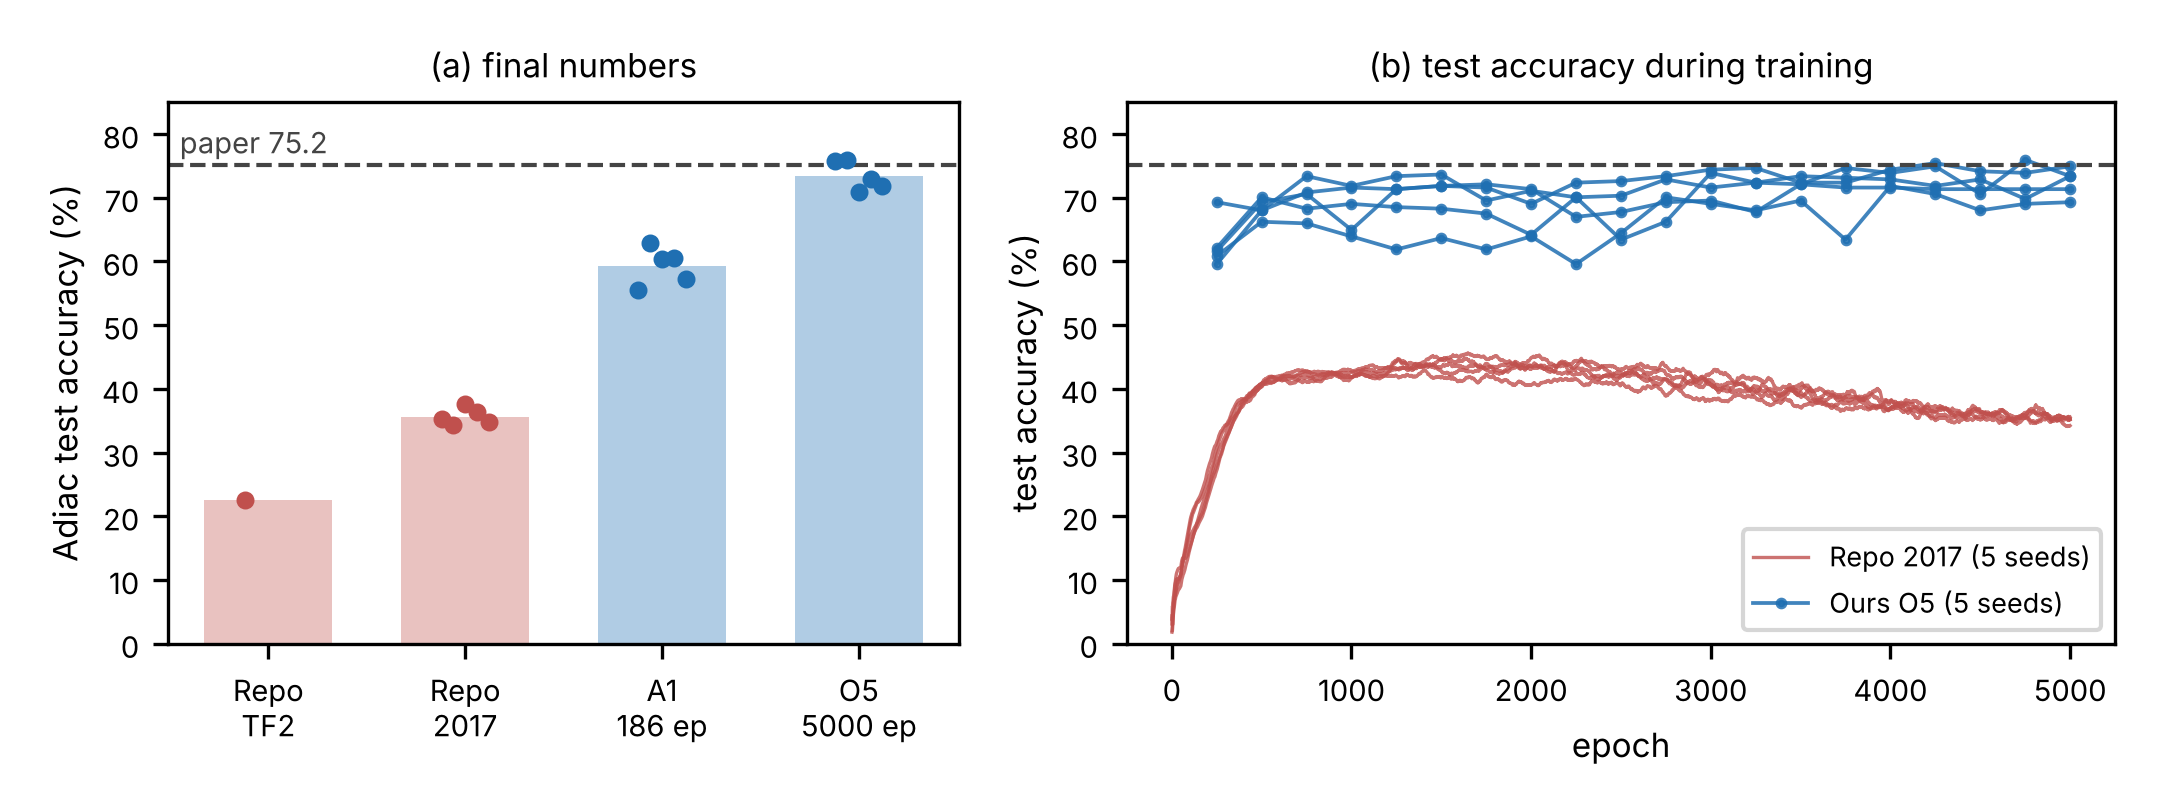
\includegraphics[width=0.78\textwidth]{mlp_figure.png}}
\caption{MLP on Adiac. (a) Test accuracy of each setting (bars: mean, dots: seeds; dashed: paper). (b) Test accuracy during training: published code in the 2017 environment (smoothed over 50 epochs) and our compact MLP (values logged every 250 epochs).}
\label{fig:mlp}
\end{figure*}

\textbf{What the numbers also show.} (i) The lowest-training-loss epochs of O5 are 4750 to 4994 of 5000, so the paper's rule is almost the same as taking the last epoch (mean 72.48\%). Our best-test-epoch diagnostic averages 75.19\%, which we do not use. (ii) Accuracy and loss decouple: the test loss at the selected epoch is 4.92 on average against 1.56 after 186 epochs, because the network fits the training set to 99--100\% and becomes overconfident, while the test accuracy still rises. (iii) The seed matters: for seed 813308 the best test epoch was 1668 (74.17\%), but the selected epoch 4823 gave 70.84\%.

\textbf{Limits of this improvement.} It was developed and tested on one dataset (Adiac) and five seeds. We changed the architecture, the optimiser and the regularisation, so this is an optimised alternative, not a reproduction of the authors' MLP. We have not shown that it also helps on the other datasets.

\section{FCN Baseline}
The FCN has three convolution blocks (128, 256 and 128 filters, kernel sizes 8, 5 and 3) with batch normalisation and ReLU, global average pooling and a softmax layer, trained with Adam (learning rate 0.001); the authors' script uses 2000 epochs and a learning rate that halves after 50 epochs without improvement. The script needs the same kind of patches as ResNet, and its class activation map code must be disabled because it uses a removed backend function. It also contains the same label rescaling as the ResNet script (Section~\ref{sec:resnet}). Our runs use an FCN rebuilt with true one-dimensional kernels (270,501 parameters on Adiac), the paper's selection rule, and seeds 0 to 4 on Adiac and 0 to 2 elsewhere.

\textbf{Results.} At 300 epochs the FCN is far from the paper on Adiac (0.379 against 0.143), Beef, FaceFour, ECGFiveDays and OliveOil, but agrees on GunPoint and SwedishLeaf (Table~\ref{tab:fcn}). At 2000 epochs, the authors' length, Adiac and OliveOil improve a lot (0.379 to 0.207, 0.767 to 0.211), which shows that the FCN is undertrained at 300 epochs, unlike ResNet. Beef, FaceFour and ECGFiveDays do not improve (0.444 to 0.456, 0.246 to 0.295, 0.160 to 0.214), and the standard deviations over three seeds reach 0.10. We do not reproduce the published FCN error on Adiac (0.143) even with 2000 epochs.

\begin{table}[htbp]
\caption{FCN test error, paper against our runs. Mean $\pm$ standard deviation over seeds (300 epochs: Adiac $n=5$, others $n=3$; 2000 epochs: $n=3$).}
\begin{center}
\footnotesize
\setlength{\tabcolsep}{3pt}
\begin{tabular}{|l|c|c|c|}
\hline
\textbf{Dataset} & \textbf{Paper} & \textbf{300 epochs} & \textbf{2000 epochs} \\
\hline
Adiac & 0.143 & 0.379 $\pm$ 0.044 & 0.207 $\pm$ 0.049 \\
Beef & 0.250 & 0.444 $\pm$ 0.019 & 0.456 $\pm$ 0.051 \\
ECGFiveDays & 0.015 & 0.160 $\pm$ 0.044 & 0.214 $\pm$ 0.100 \\
FaceFour & 0.068 & 0.246 $\pm$ 0.093 & 0.295 $\pm$ 0.099 \\
GunPoint & 0.000 & 0.011 $\pm$ 0.019 & -- \\
OliveOil & 0.167 & 0.767 $\pm$ 0.145 & 0.211 $\pm$ 0.051 \\
SwedishLeaf & 0.034 & 0.036 $\pm$ 0.004 & -- \\
\hline
\end{tabular}
\label{tab:fcn}
\end{center}
\end{table}

\textbf{Attempted improvement: squeeze-and-excitation and label smoothing.} We added squeeze-and-excitation blocks~\cite{hu2018} (+24,576 parameters, +9\%) and label smoothing with 0.1~\cite{szegedy2016}, alone and together, and compared them with the baseline on seven datasets at 300 epochs with the same seeds. The paired differences have mixed signs. Over the seven datasets, a Wilcoxon test gives $p=0.27$ for squeeze-and-excitation and $p=0.94$ for label smoothing with the paper's selection rule ($p=0.94$ for both with the last epoch). The combination is worse on all seven datasets ($p=0.016$). Since the baseline is undertrained at 300 epochs, the ablation cannot show whether the blocks help a converged network, and we do not claim a gain. A 2000-epoch ablation was not completed \todo{replace with results if the 2000-epoch ablation finished}.

\textbf{A methodological lesson.} Our first version of this experiment chose the checkpoint with the highest test accuracy, which leaks the test set into the result. We replaced it with the paper's training-loss rule and a protocol that never reads the test set for selection (\texttt{src/fcn\_variants.py}).

\section{ResNet Baseline}\label{sec:resnet}
\subsection{Model and Reproduction}
The ResNet has three residual blocks of three convolutions each, with 64, 128 and 128 filters and kernel sizes 8, 5 and 3, batch normalisation and ReLU after each convolution, global average pooling and a softmax layer, following He et al.~\cite{he2015}. It is trained with Adam (learning rate 0.001). The published script needs three edits to run (the renamed \texttt{nb\_epoch} and \texttt{val\_acc}, and the \texttt{idxmin} call); we kept the original and ran a patched copy.

A first Adiac run with the authors' settings (1500 epochs, no seed control) gave an error of 0.1765 against 0.174 in the paper. A runner script then fixed the dataset, epochs and seed, and recorded the error at the lowest-training-loss epoch. We ran Adiac with five seeds at 300 epochs and two seeds at 1500 epochs, and ten further datasets at 300 epochs (three seeds for Beef, OliveOil and ECGFiveDays, one seed for the others).

\subsection{Results}
Seven of the nine small datasets in Table~\ref{tab:resnet} agree with the paper within two test series or are better (OliveOil, FaceFour, GunPoint, Trace, TwoLeadECG, SonyAIBO, ItalyPower). Adiac is 16 test series above the paper (mean of five seeds), 50words 23, Beef 11 and ECGFiveDays 110.

\begin{table}[htbp]
\caption{ResNet test error, paper against our runs (300 epochs). Mean $\pm$ standard deviation over seeds (Adiac $n=5$; Beef, OliveOil, ECGFiveDays $n=3$; others $n=1$). Gap: our $k\times k$ mean minus the paper, in test series.}
\begin{center}
\footnotesize
\setlength{\tabcolsep}{3pt}
\begin{tabular}{|l|c|c|c|c|}
\hline
\textbf{Dataset} & \textbf{Paper} & \textbf{Ours $k\times k$} & \textbf{Ours $k\times 1$} & \textbf{Gap} \\
\hline
Adiac & 0.174 & 0.215 $\pm$ 0.028 & 0.200 $\pm$ 0.036 & +16 \\
50words$^{\mathrm{a}}$ & 0.273 & 0.323 & -- & +23 \\
Beef & 0.233 & 0.589 $\pm$ 0.051 & 0.567 $\pm$ 0.058 & +11 \\
OliveOil & 0.133 & 0.200 $\pm$ 0.116 & 0.189 $\pm$ 0.069 & +2 \\
ECGFiveDays & 0.045 & 0.173 $\pm$ 0.104 & 0.114 $\pm$ 0.066 & +110 \\
FaceFour & 0.068 & 0.080 & -- & +1 \\
GunPoint & 0.007 & 0.013 & -- & +1 \\
Trace & 0.000 & 0.020 & -- & +2 \\
TwoLeadECG & 0.000 & 0.001 & -- & +1 \\
SonyAIBO & 0.015 & 0.015 & -- & 0 \\
ItalyPower & 0.040 & 0.036 & -- & $-$4 \\
\hline
\multicolumn{5}{l}{$^{\mathrm{a}}$Labels as published; with corrected labels 0.314.}
\end{tabular}
\label{tab:resnet}
\end{center}
\end{table}

\begin{figure*}[t]
\centerline{\includegraphics[width=0.95\textwidth]{resnet_figure.png}}
\caption{Left: ResNet test error per dataset for the paper (cross), our first Adiac run with 1500 epochs (star) and our 300-epoch runs with square and one-dimensional kernels (mean and standard deviation over seeds). Right: number of parameters of the two kernel layouts.}
\label{fig:resnet}
\end{figure*}

\subsection{Lessons Learned}
\textbf{The first result matches, but it is one draw.} Controlled seeds gave 0.2455, 0.2430 and 0.1816 (seeds 0 to 2) and a mean of $0.215\pm0.028$ over five seeds. The paper's value lies at the favourable end of this spread, which is consistent with a favourable single run; five seeds cannot exclude a small systematic gap, for example from changed library defaults.

\textbf{Longer training did not help ResNet.} With the same seeds, 1500 epochs gave 0.2506 and 0.1893 against 0.2430 and 0.1816 at 300 epochs, while one run took about 129 minutes instead of 24. The seed mattered much more than the epochs, so we used 300 epochs elsewhere.

\textbf{Undocumented settings.} The paper does not state the number of epochs (1500 in the code), the batch size ($\min(n/10,16)$), a learning rate schedule (halving after 50 epochs without improvement, down to $10^{-4}$), a batch normalisation layer on the raw input, or the projection shortcut ($1\times1$ convolution with batch normalisation in all three blocks, whereas the text gives a plain sum). The code seeds only NumPy, so TensorFlow runs are not repeatable, and it passes the test set as validation data, so the logged validation metrics are test metrics.

\textbf{A label bug on 50words.} The code rescales labels with floating-point arithmetic and truncates them. We checked all 85 datasets: only 50words is affected, where 50 classes become 44 and 27\% of the labels (124 of 450 training and 121 of 455 test series) are wrong. The FCN script has the same code. In one paired run the error was 0.3231 with the published labels and 0.3143 with corrected labels, a difference of four test series that is within seed noise.

\textbf{Unexplained gaps.} Beef (0.589 against 0.233) and ECGFiveDays (0.173 against 0.045) stay far above the paper for every seed, and one-dimensional kernels do not fix them. Training set size alone does not explain it, because OliveOil and TwoLeadECG have similarly small training sets and agree with the paper. We did not test changed library defaults at batch sizes of two or three, or favourable single runs in the paper, as causes.

\subsection{Improvement: One-Dimensional Kernels}
The code uses \texttt{Conv2D(f, k, 1)} on inputs of shape (length, 1, 1). In Keras~1 this meant a $k\times1$ kernel, but in current Keras the third argument is the stride, so the layers use $k\times k$ kernels on an input one element wide. The function is equivalent, because the extra columns only see padding, but the network carries many unused weights. We rebuilt the same architecture with $k\times1$ kernels. The parameters drop from 2,866,149 to 527,845 (5.4 times fewer), and a benchmark epoch takes 0.68 s instead of 2.67 s. Real runs are 3.4 times faster on Adiac (7.0 against 23.9 minutes) and 2.6 to 3.7 times on Beef, OliveOil and ECGFiveDays.

Accuracy does not change detectably. On Adiac the mean error over five seeds is $0.200\pm0.036$ against $0.215\pm0.028$ (Welch $t\approx0.8$), and the paired differences for seeds 0 to 2 have mixed signs ($-0.046$, $+0.008$, $-0.026$). The same holds on Beef, OliveOil and ECGFiveDays, where differences are below one standard deviation. Two of five $k\times1$ seeds (0.156 and 0.1765) reach or beat the paper's 0.174.

\section{Discussion: What Holds Up}
Table~\ref{tab:summary} summarises Adiac. The ranking of the paper survives: the two convolutional models are clearly better than the MLP, and ResNet is close to the published value. The absolute numbers do not survive equally well.

\begin{table}[htbp]
\caption{Adiac test error: paper, the published code in our hands, and our improved version.}
\begin{center}
\footnotesize
\setlength{\tabcolsep}{3pt}
\begin{tabular}{|l|c|c|c|}
\hline
\textbf{Model} & \textbf{Paper} & \textbf{Published code} & \textbf{Ours improved} \\
\hline
MLP & 0.248 & 0.644 & 0.265 (128 units) \\
FCN & 0.143 & 0.379 / 0.207$^{\mathrm{b}}$ & no gain (SE, LS) \\
ResNet & 0.174 & 0.215 & 0.200 ($k\times1$, 5.4$\times$ smaller) \\
\hline
\multicolumn{4}{l}{\scriptsize MLP: 2017 environment; FCN$^{\mathrm{b}}$: 300 / 2000 epochs; ResNet: 300 epochs.}
\end{tabular}
\label{tab:summary}
\end{center}
\end{table}

\textbf{What works as published.} The architectures train end to end on raw series, and on easy datasets (GunPoint, Trace, TwoLeadECG, SonyAIBO, ItalyPower) our errors agree with the paper within two test series.

\textbf{What does not.} (i) The code does not run on current libraries, and its behaviour depends on library defaults (Adadelta learning rate, the meaning of the third \texttt{Conv2D} argument). (ii) The MLP result is not reproducible with the repository, in either of two environments. (iii) The FCN error on Adiac is not reached, and its 300-epoch results are misleading because the network is undertrained. (iv) One run per dataset hides a spread of several points (ResNet on Adiac, $\pm0.028$; FCN on small datasets up to $\pm0.15$). (v) Important settings (epochs, schedule, input normalisation, shortcut type) are missing from the paper, and one script has a label bug.

\textbf{Other findings.} The paper's selection rule is almost the last epoch when training runs long, so it behaves like a fixed training length; it still evaluates on the test set at every epoch, which tempts users to select on it, as our first FCN script did. Low test loss and high test accuracy can disagree (MLP). Model size can be cut a lot without loss (ResNet 5.4 times, MLP 22 times), which suggests that the published networks are larger than necessary for these datasets.

\section{Conclusion and Repository}
The paper's main message, that simple end-to-end networks are strong baselines, mostly survives for ResNet and FCN on small datasets, but its exact numbers are not safe to use as targets: they depend on one run, undocumented settings and library behaviour, and the MLP could not be reproduced at all. Our improvements show that a compact MLP and one-dimensional ResNet kernels keep or recover accuracy with far fewer parameters, while SE blocks and label smoothing did not help FCN in our budget. Limitations are the CPU-only budget, one improved dataset for the MLP, three to five seeds, and untested explanations for the Beef, ECGFiveDays and MLP gaps. The repository \texttt{github.com/Atharva-More/Network} contains the untouched original code, the patched copies and diffs, the scripts with one command per result, the logs, and the paper-versus-ours tables (\texttt{results/}).

\section*{Workplan and Contributions}
\begin{center}
\footnotesize
\setlength{\tabcolsep}{3pt}
\begin{tabular}{|p{2.0cm}|p{5.9cm}|}
\hline
\textbf{Member} & \textbf{Contribution} \\
\hline
Atharva More & Environment and repository setup; ResNet reproduction (seed, epoch and dataset runs); label bug scan over 85 datasets; one-dimensional kernel improvement; FCN squeeze-and-excitation and label smoothing ablation; paper-versus-ours tables and figures. \\
Payal KR, Vansh & MLP and FCN reproduction; MLP architecture search, 186-epoch and 5000-epoch evaluation. \todo{assign exactly who did which part} \\
\hline
\end{tabular}
\end{center}
Reproduction commands for every result are listed in the repository README.

\begin{thebibliography}{00}
\bibitem{wang2016} Z. Wang, W. Yan, and T. Oates, ``Time series classification from scratch with deep neural networks: A strong baseline,'' in \textit{Proc. IJCNN}, 2017, pp. 1578--1585 (arXiv:1611.06455).
\bibitem{he2015} K. He, X. Zhang, S. Ren, and J. Sun, ``Deep residual learning for image recognition,'' in \textit{Proc. CVPR}, 2016, pp. 770--778.
\bibitem{ucr2015} Y. Chen, E. Keogh, B. Hu, N. Begum, A. Bagnall, A. Mueen, and G. Batista, ``The UCR time series classification archive,'' 2015.
\bibitem{bagnall2017} A. Bagnall, J. Lines, A. Bostrom, J. Large, and E. Keogh, ``The great time series classification bake off,'' \textit{Data Min. Knowl. Discov.}, vol. 31, no. 3, pp. 606--660, 2017.
\bibitem{fawaz2019} H. Ismail Fawaz, G. Forestier, J. Weber, L. Idoumghar, and P.-A. Muller, ``Deep learning for time series classification: a review,'' \textit{Data Min. Knowl. Discov.}, vol. 33, no. 4, pp. 917--963, 2019.
\bibitem{hu2018} J. Hu, L. Shen, and G. Sun, ``Squeeze-and-excitation networks,'' in \textit{Proc. CVPR}, 2018, pp. 7132--7141.
\bibitem{szegedy2016} C. Szegedy, V. Vanhoucke, S. Ioffe, J. Shlens, and Z. Wojna, ``Rethinking the Inception architecture for computer vision,'' in \textit{Proc. CVPR}, 2016, pp. 2818--2826.
\end{thebibliography}

\end{document}
